\clearpage
\section{Related Work}
\label{sec:related_work}

Urban planning and transportation is evolving rapidly in response to the increasing emphasis on sustainability and proximity-based accessibility. 
This section consists of a comprehensive review of existing literature by focusing on key areas such as accessibility analysis, routing algorithms, and the integration of public transport data with street network data. 
The objective is to build a theoretical foundation for the development of methodologies aimed at optimizing urban accessibility. 
The first part of this section explores the paradigm shift from traditional mobility-based planning to accessibility-based planning.
This shift is crucial in addressing modern urban challenges such as reducing greenhouse gas emissions and promoting sustainable transportation. 
Subsequently, we examine various routing algorithms that are central to effectively assess accessibility. 
These include established algorithms like Dijkstra, Multi-Label-Correcting (MLC), and innovative approaches tailored for public transport networks, such as RAPTOR, McRAPTOR, and Multimodal Multicriteria RAPTOR (MCR). 
Furthermore, the integration of public transport data, primarily through the General Transit Feed Specification (GTFS), and street network data sourced from OpenStreetMap (OSM) are discussed. 
This integration is vital for a realistic simulation of urban dynamics and to enable the reproducibility of our results. 
Finally, we address the significance of multimodality and intermodality in urban planning.
This is important because considering diverse transport modes, including bicycle sharing and public transport, and investigating their synergies are vital to retrieve a holistic view of urban accessibility.
This literature review sets the stage for the subsequent sections, where we develop and test a new tool for accessibility-based planning, incorporating multimodal and intermodal transport options.

% \subsection{Accessibility Analysis}
% \label{subsec:accessibility_analysis}
% TODO: insert another intro sentence

\subsection{Accessibility-Based Planning}
\label{subsec:accessibility_based_planning}

Traditional mobility-based planning primarily focuses on reducing congestion and facilitating movement, often prioritizing automobile travel \cite{proffittAccessibilityPlanningAmerican2019}.
However, this approach is becoming more and more out-of-date, as modern challenges like reducing emissions of greenhouse gases are not properly addressed by it.
This is where accessibility-based planning comes into play, which focuses on planning cities in a way that provides residents with fast access to all important services \cite{proffittAccessibilityPlanningAmerican2019}.
This shift foregrounds accessibility as the primary goal, rather than merely focusing on mobility, recognizing that mobility is a means to an end and not the ultimate objective in urban planning. 

\cite{geursAccessibilityEvaluationLanduse2004a} describe four types of accessibility-based planning, seen in Table \ref{tab:accessibility_measures}.
Infrastructure-Based Accessibility is an approach that evaluates the performance and service level of transportation infrastructure.
It involves an analysis of various factors such as the levels of congestion and average travel speeds. 
The primary goal of this approach is to optimize the physical layout and capacity of transport networks to improve access to various destinations.
Even though, \cite{geursAccessibilityEvaluationLanduse2004a} describe this as an accessibility-based approach, it more closely resembles the traditional mobility-based approach.
Location-Based or Place-Based Accessibility focuses on the accessibility of essential services or employment opportunities within certain travel time or cost limits. 
This method calculates the number of critical destinations, such as schools, hospitals, or workplaces, that are reachable within a reasonable commute. It emphasizes the spatial distribution of resources and services.
Person-Based Accessibility centers on the individual’s experience in accessing various activities. This perspective acknowledges that accessibility can vary greatly based on personal factors like age, income, or physical ability. It aims to tailor urban planning to address diverse personal needs and constraints, considering personal travel patterns and individual circumstances.
Utility-Based Accessibility evaluates the economic benefits of transportation investments. 
This approach focuses on the returns of such investments in terms of improved accessibility and their overall utility to the community. 
It includes considerations of how transportation improvements can enhance the quality of life and economic opportunities for residents.

\begin{table}[ht]
\centering
\caption{Categories of Accessibility-Based Planning Measures}
\label{tab:accessibility_measures}
\begin{tabular}{|l|l|l|}
\hline
Category & Focus & Examples \\ 
\hline
Infrastructure-Based & 
  \begin{tabular}[c]{@{}l@{}}
    - Traffic performance \\
    analysis \\ 
    - Service level of \\
    infrastructure
  \end{tabular} & 
  \begin{tabular}[c]{@{}l@{}}
    - Level of congestion \\ 
    - Average travel speed
  \end{tabular} \\ 
\hline
  \begin{tabular}[c]{@{}l@{}}
      Location-Based \\
      or Place-Based
  \end{tabular} & 
  \begin{tabular}[c]{@{}l@{}}
    - Level of accessibility\\
    to locations \\ 
    - w.r.t. time \& cost
  \end{tabular} & 
  \begin{tabular}[c]{@{}l@{}}
    - Number of jobs within\\
    30 minutes \\
  \end{tabular} \\ 
\hline
Person-Based & 
  \begin{tabular}[c]{@{}l@{}}
    - Individual travel time \\ 
  \end{tabular} & 
  \begin{tabular}[c]{@{}l@{}}
    - Individual's travel time \\ 
      between activities
  \end{tabular} \\ 
\hline
Utility-Based & 
  \begin{tabular}[c]{@{}l@{}}
    - Economic benefits \\ 
  \end{tabular} & 
  \begin{tabular}[c]{@{}l@{}}
    - Transportation investments \\ 
    returns
  \end{tabular} \\ 
\hline
\end{tabular}
\end{table}


\subsection{15-Minute City}
\label{subsec:15_minute_city}


% ----INTRO OF 15 MINUTE CITY ----
A recent stream of research in the field of urban planning is the concept of the 15-minute city.
The concept is based around the idea that all essential services and amenities should be reachable within a 15-minute walking radius, reflecting a focus on reducing travel times and enhancing urban livability.
Even though, it is a concept rather than a concrete metric, the 15-minute city is closely related to location-based planning measures.
The 15-minute city concept was first introduced by Carlos Moreno, a professor at the Sorbonne University in Paris \cite{morenoIntroducing15MinuteCity2021}.
It was popularized by the mayor of Paris, Anne Hidalgo, who made it a central part of her re-election campaign \cite{gongadzeParisVision15Minute2023}.
% \cite{willberg15minuteCityAll2023} say that it is important to consider elderly people, that are not able to walk as fast as younger people.
% We could use that as an argument to why public transport needs to be considered.

% advantages
% cultivate stronger social relationsips, because people are more likely to meet \cite{allamProximityBasedPlanning15Minute2020}
% a kind of social distancing, because of primarily traveling by walking or cycling \cite{allamProximityBasedPlanning15Minute2020}
% a more environmentally sustainable mode of transport in cities, which contributes to SDG 11 \& 13 \cite{allamProximityBasedPlanning15Minute2020} \cite{papasUrbanMobilityEvolution2023}
% advantages
The 15-minute city model offers several advantages that are instrumental in shaping modern urban environments.
Primarily, it fosters the cultivation of stronger social relationships \shortcite{allamProximityBasedPlanning15Minute2020}.
In a city where essential amenities are within a 15-minute walking or cycling radius, residents are more likely to encounter each other regularly. 
This frequent interaction fosters community bonds and a sense of belonging which is beneficial for urban livability.
Additionally, this model inevitably promotes a unique form of social distancing. 
As residents primarily travel by walking or cycling, there's a natural reduction in the gathering of large crowds, typically seen in mass transit systems. 
This not only aids in maintaining public health standards but also diminishes the stress often associated with crowded urban transportation \cite{allamProximityBasedPlanning15Minute2020}.
Moreover, the shift towards walking and cycling represents a more environmentally sustainable mode of urban transport. 
This transition aligns closely with Sustainable Development Goals 11 and 13, which advocate for sustainable cities and communities, and taking urgent action to combat climate change, respectively. 
By reducing reliance on motorized vehicles, the 15-minute city concept contributes to lowering carbon emissions and minimizing the overall environmental impact of urban areas \shortcite{allamProximityBasedPlanning15Minute2020, papasUrbanMobilityEvolution2023}.

Furthermore, an important economic benefit of the 15-minute city is the significant reduction in traffic. 
This decrease in traffic congestion not only enhances the efficiency of urban transport systems but also leads to economic savings for both individuals and the city as a whole, due to lower transportation costs and time savings.
This aspect underscores the economic viability of the 15-minute city model in creating more efficient and cost-effective urban environments \shortcite{allamProximityBasedPlanning15Minute2020, papasUrbanMobilityEvolution2023}.

In addition, developing cities around the 15-minute city concept can play a crucial role in reducing social inequalities. 
Since walking is a free mode of transport, it becomes an accessible option for all socioeconomic groups, thereby leveling the playing field for urban residents. 
This inclusivity is central to the concept's appeal and effectiveness \cite{weng15minuteWalkableNeighborhoods2019b} \cite{gustafsonExaminingSpatialChange2022}.
However, when incorporating other fare-based modes of transport, such as bicycle sharing, it is vital to consider the fares and their impact on accessibility and equity. 
This consideration is a key reason for the adoption of multi-objective approaches in urban planning, ensuring that the benefits of the 15-minute city are equitably distributed across all sections of society.


\subsection{Accessibility Metrics Based on the 15-Minute City}
\label{subsec:accessibility_metrics_based_on_the_15_minute_city}

% --- NEXI ---
Quantitative studies have developed various ways to measure how well cities match the idea of the 15-minute city concept,  by developing metrics that encapsulate this principle.  
\cite{olivariAreItalianCities2023} contribute to this research by creating the NExt proXimity Index (NEXI), which has two components: the NEXI-Minutes and the NEXI-Global. 
The NEXI-Minutes looks at the accessibility of various urban amenities, ranging from educational institutions to entertainment venues and grocery stores by calculating the time needed to reach the closest facility within each category.
Complementing this, the NEXI-Global, inspired by the Walk Score method \cite{WalkScoreMethodology}, combines these individual times through a weighted average into an overall score giving a holistic view of the accessibility of a city.

NEXI is unique because it is both global and local - globally applicable due to its reliance on OpenStreetMap data, yet sufficiently detailed to assess local conditions.
This has been proven by applying it all over Italy, where it's showcased on an interactive map through a hexagonal grid that makes it easy to see which areas are doing well and need improvement.
The significance of the NEXI, as underscored by \cite{olivariAreItalianCities2023}, is its role in enabling data-driven policy-making, to develop cities in the fashion of the 15-minute city framework. 
Therefore, their index enables accessibility-based planning.
Despite the potential benefits, \cite{olivariAreItalianCities2023} acknowledge the challenges in realizing the 15-minute city model, notably the substantial investments and strategic planning required. 

However, there are some limitations in the NEXI metrics. 
The NEXI-Minutes offers separate metrics for each category, which may lead to a fragmented understanding of urban accessibility. 
This multi-metric approach can make comprehensive evaluation challenging. 
In addition, the NEXI-Global, while aggregating these categories, introduces complexity through its weighted scoring system. 
The weights are hard for humans to evaluate and the score from 0 to 100 disconnects the metric from the intuitive meaning of minutes.
This makes it more difficult for urban planners and policymakers to interpret and utilize the results effectively. 
These factors suggest a need for refinement in the NEXI methodology to enhance its practical utility in urban development and planning.


% --- CITYACCESSMAPS ---
Another study that deals with an accessibility metric built on the concept of the 15-minute city by \cite{nicolettiDisadvantagedCommunitiesHave2023} explores the connection between urban infrastructure and social inequality. 
The researchers developed an open, data-driven framework to analyze how different communities within cities access essential services, and they discovered that access to urban amenities like healthcare, education, and transportation is not evenly distributed. 
In particular, communities with more minorities, lower incomes, and fewer university-educated individuals often have less access to these important services.
The study examined over 50 types of amenities across 54 cities worldwide and found a common pattern: in all cities, access to infrastructure followed a log-normal distribution, indicating that disparities in accessibility are linked to the city's growth. 
This pattern was consistent even when considering various socio-economic factors.

The framework introduced by \cite{nicolettiDisadvantagedCommunitiesHave2023} is flexible and adaptable, allowing city planners to tailor it to local needs and priorities. 
It's a tool that can help identify which groups in a city are most affected by inequality in access to services. 
Similar to \cite{olivariAreItalianCities2023} they emphasize the role of open data to guide urban planning and policy.
While \cite{olivariAreItalianCities2023} simply provide a tool to measure accessibility and leave the analysis and interpretation to practitioners, \cite{nicolettiDisadvantagedCommunitiesHave2023} directly reveal the disparities in accessibility and provide a framework to analyze them.

% --- critique on both ---
However, the computation of travel time by all previously named authors is based on walking simulations. 
This fails to capture the reality of urban mobility, which consists of various modes of transport, such as public transport, cycling, and driving.
The potential benefits of infrastructure such as dedicated bicycle lanes, bicycle sharing systems, and highly available public transport are thus not reflected within the research of \cite{olivariAreItalianCities2023} and \cite{nicolettiDisadvantagedCommunitiesHave2023}.
To provide a more accurate measure, we propose to enhance the computation of accessibility by integrating a multimodal accessibility metric that accounts for these various transportation methods and their respective infrastructural elements.

% --- barcelona
% TODO: this is written like shit
\cite{ferrer-ortizBarcelona15MinuteCity2022} calculate whether a certain area has access to a certain category within 15 minutes for Barcelona
They derive their categories from the six 15-minute city "urban social functions" defined by Moreno.
However, they only deal with a subset of four, namely care, education, provisioning and entertainment.

% --- outro & transition to next algorithms ---
While the NEXI and the open data-driven framework are the most prevalent examples for metrics based on the 15-minute city concept, they are not without limitations.
The NEXI's fragmented multi-metric approach and its complex weighted scoring system can hinder practical interpretation and application.
Similarly, the exclusive focus on walking in travel time computations overlooks the diverse modes of urban transport, such as cycling and public transportation.
Acknowledging these shortcomings, we aim to introduce a novel multimodal accessibility metric, which we introduce in Section \ref{subsec:metric}.
This proposed metric will encompass a broader spectrum of transportation methods, thereby providing a more accurate and comprehensive evaluation of urban accessibility for effective urban planning.

\subsection{Routing Algorithms}
\label{subsec:routing_algorithms}

Following the discussion of accessibility metrics and their application in urban planning, particularly in the context of the 15-minute city model, this subsection transitions to a vital component underpinning these metrics: routing algorithms.
The focus here is on the exploration of various routing algorithms that are instrumental in calculating the shortest and most efficient paths within urban environments. 

\subsubsection{Theoretical Backgrounds}

Before exploring the specific algorithms, it is important to understand the theoretical foundations of routing algorithms.
The primary goal of routing algorithms is to identify the optimal path between a designated origin and a specific destination.
Typically, this is captured using a graph representation:
\[ G = (V, E) \]
where $V$ represents a set of nodes (or locations) and $E$ encapsulates the set of edges, which correspond to connections between these nodes.

For each edge \( e \in E \), there's an associated weight \( w(e) \in \mathbb{R} \) that characterizes the cost of traversing it.
This cost might be determined by factors such as distance or travel time.
Consequently, the shortest path can be expressed as:
\[ \langle v_0, e_0, v_1, e_1, \dots, v_n \rangle \]
Here, \( v_0 \) denotes the origin, \( v_n \) the destination, and the edges must connect the nodes in the sequence:
\[ e_i = (v_i, v_{i+1}) \quad \text{for} \quad i \in \{0, \dots, n-1\} \]
In accessibility contexts, the primary concern frequently revolves around determining the accumulated cost, \( d(v_n) \), to reach the destination rather than the actual path.

The problem may also encompass multiple objectives, such as considering both time and monetary cost of travel.
Under these circumstances, the edge weight is represented as a vector:
\[ w(e) \in \mathbb{R}^k \]
where \( k \) stands for the total objectives count.
Unlike the simpler single-objective case with a singular optimal path, the multi-objective optimization yields a Pareto set, constituting several optimal routes.
A Pareto set refers to a set of solutions that are non-dominated by any other solution.
This means that for each solution in the Pareto set, there is no other solution that is better in all objectives.
The Pareto set represents an optimal trade-off among the different objectives, where improving one aspect would worsen another.
For example, a Pareto set could contain multiple paths, where one path is faster, but more expensive, while another path is slower, but cheaper.

The value of these paths is depicted using a label:
\[ l \in \mathbb{R}^k \]
where \( l_i \in \mathbb{R} \) denotes the value for the \( i \)-th objective.
This label can be thought of as a multidimensional extension of \( d(v_n) \) from the single-objective scenario.
The Pareto set associated with destination node \( v_n \) is often termed as a bag, expressed as \( B(v_n) \), comprising labels that are not dominated by each other.
Domination is defined as follows: \( l' \) dominates \( l \) if \( l'_i \leq l_i \) for all \( i \in \{1, \dots, k\} \) and \( l'_i < l_i \) for at least one \( i \in \{1, \dots, k\} \).
Intuitively, this means that \( l' \) is at least as good as \( l \) in all objectives and strictly better in at least one objective.

The goal of routing algorithms used in accessibility analysis is finding the distance in the single objective case and the bag in the multi objective case, often discarding the actual paths.
For accessibility analysis routing algorithms are often altered to not find the optimal path(s) between two nodes, referred to as one-to-one query, but the path from a single origin to all other nodes in the network, which we call one-to-all query.

\subsubsection{Dijkstra}
\label{subsubsec:dijkstra}
The most straightforward approach to compute the shortest paths in a graph is the Dijkstra algorithm \cite{dijkstra1959note}.
Dijkstra's algorithm initiates at a designated start node \( s \in V \) and employs a priority queue to systematically determine the shortest path to each subsequent node \( v \in V \).
Initially, the distance to the start node \( s \) is set to zero, while the distances to all other nodes are set to infinity.
In each iteration, the algorithm dequeues the node \( u \) with the smallest known distance from the priority queue.
It then examines each outgoing edge \( e = (u, v) \) from \( u \), updating the distance to \( v \) if a shorter path through \( u \) is discovered.
Specifically, if \( \text{dist}(u) + w(e) < \text{dist}(v) \), then \( \text{dist}(v) \) is updated to \( \text{dist}(u) + w(e) \), and \( v \) is enqueued into the priority queue for future exploration.
The node \( u \) is marked as visited by adding it to the set \( V_{\text{visited}} \).
Depending on the goal, the algorithm terminates either when the destination node is dequeued (one-to-one) or when the priority queue is empty (one-to-all).


However, this simple approach has multiple problems.
Firstly, the Dijkstra algorithm is not able to handle multiple criteria.
Secondly, the runtime of Dijkstra's algorithm is \( O(|E| + |V| \log |V|) \), which is too slow for large graphs.

\subsubsection{MLC}
\label{subsubsec:mlc}

The Multi-Label-Correcting (MLC) \shortcite{hansenBicriterionPathProblems1980} algorithm is an extension of Dijkstra's algorithm to handle multi-objective scenarios.
As mentioned in Section \ref{subsec:routing_algorithms} in the multi-objective case we try to find the bag of the destination node.
Specifically, for \(k\) criteria, each node \(v\) retains a bag of \(k\)-dimensional labels. Such a list encapsulates a set of Pareto-optimal paths from the starting node to \(v\).
Similarly to Dijkstra's algorithm, MLC initializes all nodes with an empty bag, except for the start node, which is initialized with a label of \( (0, \dots, 0) \in \mathbb{R}^k \).
Each iteration extracts the lexicographically smallest label, as opposed to selecting the node with the minimum distance.
When a label is extracted and \(v\) is its corresponding node, updates are made for all connected edges \( (v, w) \).
The update process consists of comparing a newly generated tentative label against all labels within the bag of \(w\).
This new label is only inserted into the bag if it isn't dominated by any existing label.
Conversely, any label now dominated by the new entry is removed.
Each time a label is inserted into a bag, it is also inserted into the priority queue.
The algorithm terminates when the priority queue is empty.

The major drawback of the MLC algorithm is its runtime, which is even slower than Dijkstra's algorithm, because each node can be visited multiple times.


\subsubsection{Graph-based Algorithms in Public Transport}
\label{subsubsec:graph_based_algorithms_in_public_transport}


In the context of accessibility analysis the previously mentioned algorithms can be used directly for walking, cycling and driving networks.
%To do so the network is represented as a graph and the edge weights are set to the travel time.
%It is also possible to represent multi-modal networks as a graph, connecting the different graphs with transfer edges.
%These transfer edges repre
However, public transport networks pose a challenge, since they contain time-dependent information, such as the departure time of a trip.
To overcome this challenge two different approaches are commonly used, the time-expanded and the time-dependent approach, as explained by \cite{muller-hannemannTimetableInformationModels2007}.
While enabling the use of graph-based algorithms to solve routing in time-dependent transport networks, both approaches result in huge graphs and therefore suffer from the previously mentioned runtime problems.

\subsubsection{RAPTOR}
\label{subsubsec:raptor}

To overcome the runtime problems of graph-based approaches, \cite{dellingRoundBasedPublicTransit2015} introduce one of the most prominent routing algorithms for public transport, called Round based Public Transit Optimized Router algorithm (RAPTOR). % which is also used by R5
Unlike traditional Dijkstra-based algorithms, RAPTOR operates in rounds, looking at each route (such as a bus line) in the network at most once per round, where one round represents a single trip.

As RAPTOR does not operate on a graph, we first introduce the problem statement.
Raptor operates on a scheduled network consisting of routes \(r\), trips \(t\), stops \(p\), and stop times that associate trips with stops.
% Next paragraph should probably be handled in the method
% Here it is important to understand the differences between what we consider as a route in RAPTOR and other algorithms and what is considered as a route in GTFS data. In GTFS data, a route can have multiple different stop sequences, let's call them paths. For example, it is almost always the case that the path and the reversed path are associated with the same route. Therefore, it is not straightforward to convert GTFS routes into routes that can be used in RAPTOR.
A route is associated with a sequence of stops \(stops(r) = \langle p_1, \dots, p_n \rangle\).
A route has multiple trips ordered by their departure time \(trips(r) = \langle t_1, \dots, t_m \rangle\).
One trip associates arrival and departure times with each stop of the route, denoted by \(arrivalTime(t, s) \in \mathbb{N}\) and \(departureTime(t, s) \in \mathbb{N}\) respectively.
% talk about time representation?
Trips of the same must not overtake each other, formally:
\[departureTime(t_i, p_j) \leq arrivalTime(t_{i+1}, p_j)\]
for all \(i \in \{1, \dots, m-1\}\) and \(j \in \{1, \dots, n\}\).
Each stop \(p\) has a minimal exchange time \(\tau_{ch}(p) \in N\) associated with it.
Often, the exchange time is set to a fixed time \(\tau_{ch}(p) = \tau_{ch}\) for all stops \(p\).
When transferring from a trip \(t\) to another trip \(t'\) within at a stop \(p\), the exchange time has to be smaller than the difference in arrival and departure time of the two trips, formally:
\[arrivalTime(t, p) + \tau_{ch}(p) \leq departureTime(t', p) \]
In addition to transfer within stops, RAPTOR also allows footpaths.
Footpaths allow transferring from one stop to another without using public transport, therefore, they are time-independent.
Each footpath is associated with a travel time \(l(p, p')\).
The input of the RAPTOR algorithm, in addition to the previously described scheduled network, are source stop \(p_s\), and, in the case of a one-to-one query, target stop \(p_t\), as well as, the departure time at the source stop \(\tau\).

% Initialization: (l.2-l.8)
RAPTOR operates in rounds.
Before the first round, some variables are initialized.
We denote the earliest possible arrival time at iteration \(i\) with \(\tau_i(p)\) and the best earliest possible arrival time over the course of all iterations with \(\tau^\star(p)\).
For the source stop, \(\tau_p\), we set \(\tau_0(p) =\tau\) and \(\tau^\star(p) = \tau\).
For all other stops, we set \(\tau_0 = \infty\) and \(\tau^\star = \infty\).
In addition, we initialize a set of marked nodes \(M\) to only contain the source stop \(p_s\) and a set of marked route-stop pairs, denoted by \(Q\), to the empty set.
A route-stop pair is simply a tuple that contains a route and one of its stops.
The set of marked stops will contain all stops whose earliest possible arrival time has been updated in the current round.
Similarly, the set of marked route-stop pairs contains the routes of the marked stops, together with the earliest stop of that route that has been marked.


% Summary of steps
Each round consists of three major steps.
In the first step, the routes that have to be iterated are collected.
In the second step, the routes are iterated by "hopping" on their trips.
And in the third stage, potential footpaths are explored.

% Step 1: (l.9 - l.20)
First, we clear the set of marked route-stop pairs \(Q\).
Then we check the routes that are connected to each marked stop.
For each of these routes, we store the route-stop pair in \(Q\).
However, the routes in \(Q\) should be unique.
If there are two marked stops that are connected to the same route, we choose the stop that is earlier in the sequence of stops of that route.
Now, we clear the set of marked stops.

% Step  2: (l.21-l.33)
We iterate the route-stop pairs in \(Q\) visually depicted in Figure \ref{fig:raptor}.
The following step can be regarded as hopping on the earliest possible trip that we can catch of that route at that stop.
For each route-stop \((r,p)\) pair, we iterate over the stops in \(r\) in the sequence that is associated with \(r\), beginning with \(p\).
We check for the earliest possible trip that we can catch regarding the last arrival time at the current stop \(\tau_{k-1}(p)\) and the minimum exchange time \(\tau_{ch}(p)\).
If there is a trip that is possible to catch, we save it as the current trip \(t_{curr}\) and continue to iterate the stops of the route \(r\).
Now that we are on a trip, we have to check whether we need to update the earliest possible arrival time of the current stop \(\tau_k(p)\) and \(\tau^\star(p)\) by comparing the stop time of the current trip with the best earliest arrival time of that stop \(\tau^\star(p)\), formally:
\[\tau_k(p) = \min\{\tau_k(p), arrivalTime(t_{curr}, p)\}\]
% Here one optimization comes into play.
%We can also keep in mind the best earliest possible arrival time of the target stop \(\tau^\star(p_t)\).
%Whenever the current stop time is later than that, our current trip won't contribute to finding a faster route to the target stop, and we disregard the potential update.
In the case an update is necessary, we also add the current stop \(p\) to the marked stops.
Lastly, we check all marked stops for potential footpaths.
Remember: the marked stops are those for which the earliest possible arrival time was updated in this iteration.
For each footpath that is connected to a marked stop, we check whether the earliest possible arrival time of the other stop could be improved by the footpath.
If that is the case, we update the earliest arrival times and also mark that stop.
If no stops are marked, then there are no new routes to iterate, and the algorithm stops.
After termination \(\tau_k(p)\) contains the earliest possible arrival time at stop \(p\) with at most \(k\) transfers.
\begin{figure}
    \centering
    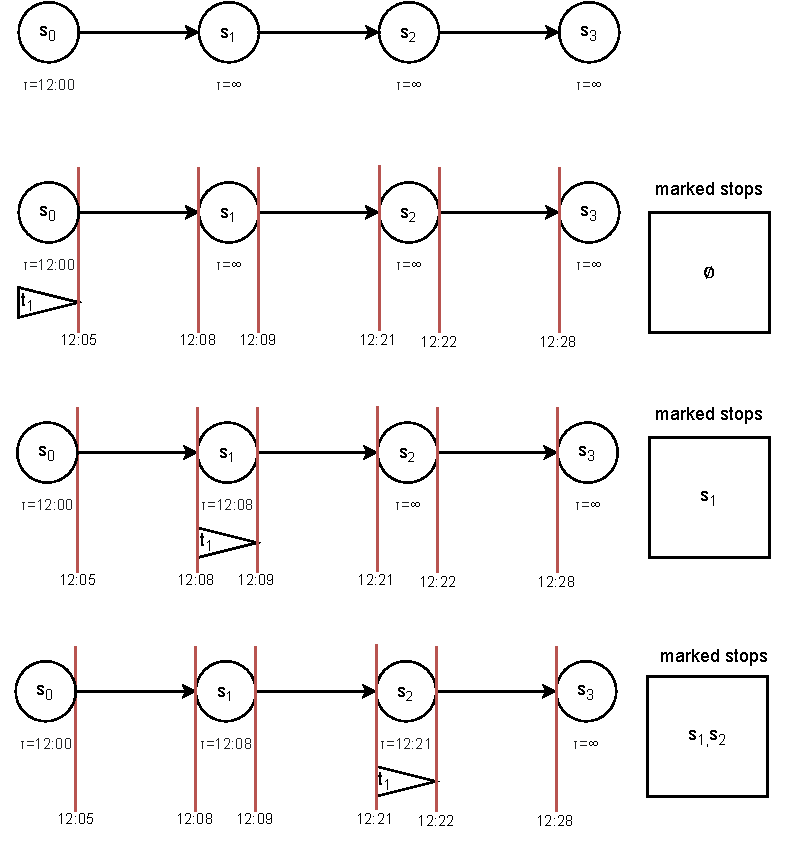
\includegraphics[width=0.70\textwidth]{Figures/related_work/raptor.pdf}
    \caption{Iterating a Route in RAPTOR}
    \label{fig:raptor}
\end{figure}

% RATPOR algorithm end
One limitation of RAPTOR is the transfer graph, which is used to represent footpaths.
The transfer graph has to be transitively closed, which means that each node has to be connected with an edge to all other nodes that can be reached from that node.
This has the advantage that in the algorithm we only have to check for direct neighbors of a stop, which is very fast.
In practice, there are many possibilities how the transfer graph could look.
First, we should note that a realistic transfer graph should be derived from a street network, as passengers should be able to walk from one stop to another using sidewalks.
To keep the transfer graph small, one could limit the maximum walking distance.
However, this may remove optimal journeys from the search space.
In general, creating the transfer graph requires some amount of preprocessing.
Therefore, finding a fitting transfer graph is challenging.
Through its round-based nature, RAPTOR is able to optimize for two criteria at the same time.
However, RAPTOR cannot incorporate more criteria and one of the criteria will always be the number of transfers.


\subsubsection{McRAPTOR}
\label{subsubsec:mcraptor}

McRAPTOR \cite{dellingRoundBasedPublicTransit2015} is an extension of RAPTOR that allows an arbitrary number of criteria.
Like MLC, McRAPTOR also uses the notion of bags containing non-dominating labels.
McRAPTOR does not pose any restrictions on how the objectives are updated during the algorithm.

The algorithm of McRAPTOR only requires slight modifications to the algorithm of RAPTOR.
In the initialization step, each stop \(p\) is assigned an empty bag, except the source stop \(p_s\), which is assigned a bag containing a starting label.
The starting label can be defined as an input, but is usually \((\tau, 0, 0, \dots, 0)\), where \(\tau\) is the departure time at the source stop.
When iterating over the route-stop pairs \((r, p)\), McRAPTOR creates a route bag that contains all labels that are in the current bag of \(p\).
In addition labels in the route bag are associated with a trip.
During creation of the route bag, each label in the route bag is associated with the first trip that is possible to catch according to the labels earliest arrival time at the current stop \(p\).
Then the route is processed, stop by stop, just like in RAPTOR.
At each stop the labels in the route bag are updated according to the current trip.
This update must include updating the earliest arrival time, but can also include updates to other criteria.
After the route has been processed, the route bag is merged into the bag of the current stop.
Merging a bag \(B_1\) into a bag \(B_2\) means that all labels in \(B_1\) that are not dominated by any label in \(B_2\) are added to \(B_2\) and all labels in \(B_2\) that are dominated by a label in \(B_1\) are removed from \(B_2\).
After the route bag has been merged into the bag of the current stop, the bag of the current stop is merged into the route bag.
Lastly, the trips that are associated with the labels in the route bag are updated according to the labels earliest arrival time at the current stop.
Each time a label is added to a stop bag, this stop is marked.
If no stop is marked after a round, the algorithm terminates.
Note that McRAPTOR allows updates to the route bags at any time during processing.
When and how the route bag should be updated fully depends on the objective and what it represents.

While McRAPTOR has a slower runtime than RAPTOR it is still magnitudes faster than MLC.
However, McRAPTOR still suffers from the same problem as RAPTOR, namely that the transfer graph is hard to compute.


\subsubsection{MCR}
\label{subsubsec:mcr}

To overcome problem of RAPTOR \cite{dellingComputingMultimodalJourneys2013} introduce Multimodal Multicriteria RAPTOR (MCR).
MCR modifies McRAPTOR so that the transfer graph must not be transitively closed.
MCR is able to directly use the street network as an input and therefore no preprocessing is necessary.
Traversing the street network directly during the algorithm has the benefit that it is possible to update the objectives between trips.
This is important if we want multiple modes of transfer, that contain free-floating vehicle sharing systems.
For example, consider the following case.
For an optimal journey a passenger has to first walk five minutes to a free-floating bicycle, with which the passenger then travels to the next stop.
There is no way to represent this in RAPTOR, because the specifics of the transfer depend on the current label, which is unknown before running the algorithm.
Therefore, it is not possible to precompute the transfer graph.

MCR as an algorithm shares substantial similarities with McRAPTOR.
The key difference in MCR is the substitution of the footpath processing step with the MLC algorithm.
Consequently, MCR can be conceptualized as an algorithm that seamlessly integrates MLC with McRAPTOR, employing each of them in an alternating manner.
The authors find that the bottleneck of MCR is the MLC step.
Therefore, they employ a technique called contraction \shortcite{geisbergerExactRoutingLarge2012} to speed up MLC.
Contraction is a preprocessing technique that reduces the size of the graph by removing nodes and adding shortcut edges.

As previously mentioned, MCR is able to use the street network as the transfer graph and requires no preprocessing.
However, when comparing the runtime of a simple query of MCR and McRAPTOR, MCR is slower, as MLC on the street network takes much more time than just checking the neighbors of a stop in the transfer graph.
Generally using MCR or McRAPTOR is a trade-off of runtime and preprocessing time.


\subsubsection{ULTRA}
\label{subsubsec:ultra}

\cite{baumUnLimitedTRAnsfersMultiModal2019} propose another algorithm building on MCR, called UnLimited TRAnsfers for Multi-Modal Route Planning (ULTRA).
ULTRA builds on the observation that extensive exploration of the transfer graph, like done in MCR, is often unnecessary for transfers between public transport trips, but is more crucial for initial and final transfers.
Therefore, they propose a preprocessing step that computes intermediate transfers that contribute to optimal journeys on the transfer graph.
They then use these precomputed transfers as the transfer graph for RAPTOR.
To account for initial and final transfers, ULTRA employs the Bucket Contraction-Hierarchies (Bucket-CH) algorithm \cite{geisbergerContractionHierarchiesFaster2008}, an efficient one-to-many approach, together with RAPTOR.

While ULTRA demonstrates a runtime improvement over MCR, it is limited to optimizing only time and the number of transfers.
Using ULTRA in an accessibility analysis setting is also unsuitable, because ULTRA runs a reverse Bucket-CH query from the end node to all stops, to compute potential final transfers.
This means that ULTRA, unlike MCR, is incompatible with one-to-many queries.

% \subsubsection{McTB}
% \label{subsubsec:mctb}

% addresses the problem that ULTRA is not suitable for more than two objectives
% However, only allows for a very specific third objective and not general ones
% \cite{potthoffFastMultimodalJourney2021}

% \subsubsection{ULTRA-PHAST}
% \label{subsubsec:ultra-phast}

% addresses the problem that ULTRA is incompatible for one-to-many queries
% However, does not allow for multiple objectives



\subsection{Public Transport Data}
\label{subsec:public_transport_data}

In order to run routing algorithms for public transport networks in practice, a common data format is needed.
The General Transit Feed Specification (GTFS) \shortcite{ReferenceGeneralTransit} serves as a standardized format for public transportation schedules and associated geographic details.
It is divided into two main components: GTFS Schedule and GTFS Realtime.
GTFS Realtime provides live transit updates.
On the other hand, GTFS Schedule offers information about routes, schedules, fares, and geographic transit details.
For our study and tool, we focus solely on GTFS Schedule and omit considerations related to GTFS Realtime.

Central to the GTFS format are several core concepts.
A route defines the overall path taken by a particular public transport service, identified by attributes like name, ID, and the mode of transport such as bus or subway.
A trip refers to a specific run of a vehicle along a route, distinguishing between different timings or sequences of service on the same route.
A stop is a specific point along a route where passengers embark or disembark.
Stops have unique IDs, names, and geographical coordinates.
Stop times specify when a vehicle is expected to be at a particular stop during its trip.
This data pinpoints both the arrival and departure timings at each stop.

% GTFS data is often distributed in plain text (.txt) files which are bundled together and compressed into a .zip file.
% This packaging makes it both compact for distribution and straightforward for developers to parse and use.

In essence, GTFS provides a comprehensive overview of a transit agency's service, covering both the spatial aspects of transit and the temporal aspects.

\subsection{Street Network Data}
\label{subsec:street_network_data}

Just as GTFS provides a standardized format for public transport schedules, the need for a consistent data format for street network information is addressed by OpenStreetMap (OSM) \shortcite{OpenStreetMap}.
OSM is a collaborative initiative that offers freely available geographic data.
This data captures various features on the Earth's surface, including roads, trails, establishments, railway stations, and more.
In the context of street networks, potentially used by routing algorithms, OSM represents roads and paths using interconnected nodes and ways.
Nodes specify distinct geographical coordinates, defined by latitude and longitude, while ways connect these nodes to define linear structures or area boundaries.
Importantly, these ways have meta-data assigned to them containing information about what vehicles can travel along them and how long they are.
In addition, OSM offers vast amounts of data about points of interest, potentially useful in accessibility analysis.
OSM is extensive, regularly updated, and most importantly freely available, which makes it indispensable for projects seeking reproducibility and generalizability.


\subsection{Importance of Multimodality \& Intermodality}
\label{subsec:importance_of_multimodality_and_intermodality}
There has been various research underlining the importance of considering multimodality and intermodality in urban planning and transportation.
Recent studies have especially highlighted the synergistic relationship between bicycle sharing and public transport systems, demonstrating their combined potential in improving urban mobility.

\shortciteA{yangImpactPublicBicyclesharing2018} illustrate the significant impact of bicycles in urban transport networks. 
Their results indicate that bicycles notably reduce average transfer times, the average journey length for passengers, and the Gini coefficient, an indicator of network efficiency. 
These findings underscore the role of bicycles in optimizing transit network performance.
Further, reinforcing this point, \shortciteA{radzimskiExploringRelationshipBikesharing2021a} identifies a positive correlation between public transport frequency and the number of bicycle trips, particularly for short and medium distances up to 3 km. 
This suggests that the availability of bicycles can complement public transport, particularly for covering the initial or final segments of a journey.
\shortciteA{murphyRoleBicyclesharingCity2015} conducted a survey in Dublin that revealed 39\% of bicycle sharing users combined this service with another mode of transport, primarily public transport (91.5\%) \shortciteA{murphyRoleBicyclesharingCity2015}. 
This indicates a high level of synergy between bicycle sharing and public transport, as commuters frequently use them together.
Similarly, \shortciteA{fishmanBikeShareSynthesis2013} reviewed literature on bicycle sharing and concluded that it is synergistic with public transport.
This synergy is further elucidated by \shortciteA{maBicycleSharingPublic2015} who, through a linear regression analysis, identified a positive correlation between public transport passenger numbers and bicycle sharing trips \shortciteA{maBicycleSharingPublic2015}. 
They suggest that bicycle sharing effectively addresses the first and last mile problem, providing a crucial link to and from transit hubs.
\shortciteA{wagnerPublicTransitRouting2017} also contributes to this discussion by demonstrating that unrestricted walking, as part of a multimodal transit system, significantly reduces travel times compared to limited walking scenarios.
However, it's also noted that computing routes with unrestricted walking is more computationally intensive.

In summary, the interplay between bicycle sharing and public transport is not just complementary but essential for urban planning and transportation.
Furthermore, incorporating unrestricted walking into transit planning, despite its computational challenges, can substantially reduce overall travel times.
Thus, considering both multimodality (the use of multiple modes of transport) and intermodality (the chaining of different modes) is vital when designing urban transportation systems and evaluating accessibility.
